% Options for packages loaded elsewhere
\PassOptionsToPackage{unicode}{hyperref}
\PassOptionsToPackage{hyphens}{url}
%
\documentclass[
]{article}
\usepackage{amsmath,amssymb}
\usepackage{iftex}
\ifPDFTeX
  \usepackage[T1]{fontenc}
  \usepackage[utf8]{inputenc}
  \usepackage{textcomp} % provide euro and other symbols
\else % if luatex or xetex
  \usepackage{unicode-math} % this also loads fontspec
  \defaultfontfeatures{Scale=MatchLowercase}
  \defaultfontfeatures[\rmfamily]{Ligatures=TeX,Scale=1}
\fi
\usepackage{lmodern}
\ifPDFTeX\else
  % xetex/luatex font selection
\fi
% Use upquote if available, for straight quotes in verbatim environments
\IfFileExists{upquote.sty}{\usepackage{upquote}}{}
\IfFileExists{microtype.sty}{% use microtype if available
  \usepackage[]{microtype}
  \UseMicrotypeSet[protrusion]{basicmath} % disable protrusion for tt fonts
}{}
\makeatletter
\@ifundefined{KOMAClassName}{% if non-KOMA class
  \IfFileExists{parskip.sty}{%
    \usepackage{parskip}
  }{% else
    \setlength{\parindent}{0pt}
    \setlength{\parskip}{6pt plus 2pt minus 1pt}}
}{% if KOMA class
  \KOMAoptions{parskip=half}}
\makeatother
\usepackage{xcolor}
\usepackage[margin=1in]{geometry}
\usepackage{graphicx}
\makeatletter
\def\maxwidth{\ifdim\Gin@nat@width>\linewidth\linewidth\else\Gin@nat@width\fi}
\def\maxheight{\ifdim\Gin@nat@height>\textheight\textheight\else\Gin@nat@height\fi}
\makeatother
% Scale images if necessary, so that they will not overflow the page
% margins by default, and it is still possible to overwrite the defaults
% using explicit options in \includegraphics[width, height, ...]{}
\setkeys{Gin}{width=\maxwidth,height=\maxheight,keepaspectratio}
% Set default figure placement to htbp
\makeatletter
\def\fps@figure{htbp}
\makeatother
\setlength{\emergencystretch}{3em} % prevent overfull lines
\providecommand{\tightlist}{%
  \setlength{\itemsep}{0pt}\setlength{\parskip}{0pt}}
\setcounter{secnumdepth}{-\maxdimen} % remove section numbering
\usepackage{graphicx}
\usepackage{float}
\usepackage{tikz}
\usepackage{xcolor}
\ifLuaTeX
  \usepackage{selnolig}  % disable illegal ligatures
\fi
\usepackage{bookmark}
\IfFileExists{xurl.sty}{\usepackage{xurl}}{} % add URL line breaks if available
\urlstyle{same}
\hypersetup{
  hidelinks,
  pdfcreator={LaTeX via pandoc}}

\author{}
\date{\vspace{-2.5em}}

\begin{document}

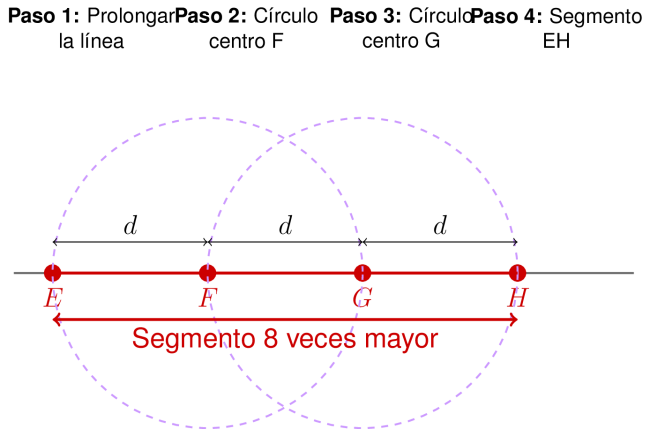
\includegraphics[width=12cm,height=\textheight]{construccion_geometrica.png}

\section{Question}\label{question}

En geometría, existe un técnica de construcción geométrica que permite
construir segmentos de longitudes específicas usando únicamente regla y
compás.

Dado un segmento \(EF\), se puede construir un nuevo segmento que tenga
4 veces la longitud de \(EF\). Para esto, se debe realizar el
procedimiento que se muestra en la figura:

\textbf{Paso 1.} Prolongar la línea que contiene el segmento \(EF\).

\textbf{Paso 2.} Trazar un círculo con centro en \(F\) que pase por el
punto \(E\) e identificar el punto \(G\), donde se cortan nuevamente la
línea y el círculo.

\textbf{Paso 3.} Trazar un nuevo círculo con centro en \(G\) que pase
por el punto \(E\) e identificar el punto \(H\), donde se cortan
nuevamente la línea y el círculo.

\textbf{Paso 4.} Crear el segmento \(EH\) uniendo el punto \(E\) y el
punto \(H\).

Si se quiere hacer un proceso similar para construir un segmento 8 veces
más grande que el segmento inicial, ¿cuál es la cantidad mínima de
círculos que se deben usar?

\subsection{Answerlist}\label{answerlist}

\begin{itemize}
\tightlist
\item
  6 círculos, porque se necesita duplicar el proceso
\item
  2 círculos, porque cada círculo amplifica por 4
\item
  3 círculos, porque cada círculo duplica la longitud del segmento
  anterior
\item
  3 círculos, porque se necesita un círculo por cada duplicación del
  ejemplo
\end{itemize}

\section{Solution}\label{solution}

Para resolver este problema, es necesario entender el patrón de la
construcción geométrica mostrada.

\textbf{Análisis del procedimiento:}

En el ejemplo mostrado: - El segmento inicial \(EF\) tiene longitud
\(d\) - Cada círculo trazado tiene radio igual a la longitud del
segmento original (\(d\)) - Cada círculo ``duplica'' la longitud del
segmento construido hasta ese momento

\textbf{Patrón de crecimiento:} - Segmento inicial: \(EF\) = \(d\) -
Después del primer círculo: \(EG\) = \(2d\) - Después del segundo
círculo: \(EH\) = \(4d\)

Por lo tanto, cada círculo duplica la longitud del segmento anterior.

\textbf{Generalización:} Para obtener un segmento \(n\) veces más largo
que el original, donde \(n\) es una potencia de 2, se necesitan
\(\log_2(n)\) círculos.

\textbf{Aplicación al problema:} Para construir un segmento 8 veces más
grande: - 8 = \(2^{3}\) - Por lo tanto, se necesitan 3 círculos

\textbf{Verificación:} - 1 círculo: \(2^1 = 2\) veces el segmento
original - 2 círculos: \(2^2 = 4\) veces el segmento original - 3
círculos: \(2^3 = 8\) veces el segmento original - 3 círculos:
\(2^{3} = 8\) veces el segmento original

\subsection{Answerlist}\label{answerlist-1}

\begin{itemize}
\tightlist
\item
  Falso. Incorrecto. 6 círculos, porque se necesita duplicar el proceso
\item
  Falso. Incorrecto. 2 círculos, porque cada círculo amplifica por 4
\item
  Verdadero. Esta es la respuesta correcta. Se necesitan 3 círculos
  porque cada círculo duplica la longitud y 8 = 2\^{} 3 .
\item
  Falso. Incorrecto. 3 círculos, porque se necesita un círculo por cada
  duplicación del ejemplo
\end{itemize}

\section{Meta-information}\label{meta-information}

exname: Construcción geométrica de segmentos con regla y compás extype:
schoice exsolution: 0010 exshuffle: TRUE exsection:
Geometría/Construcciones geométricas

\end{document}
